\section{Prologue}

After finishing the work on the \ce{Be+ + H2O} reaction, we turned our attention to focus more on branching ratios. Getting rate constants was troublesome given the requirement of having an absolute pressure measurement, while branching ratios measurements can be obtained through a single TOF trace. With our fuller understanding of the \ce{Be+ + H2O} reaction network, we focused on reaction \ref{r: Be(S)+H2O->BeOH}, for Hua Guo's group at UNM had calculated a full ground state PES. To capitalize on this, we turned to the question of whether or not there are dynamics hidden in the reaction pathway that can be seen via deuteration of \ce{H2O}.

\section{Introduction}

Together, isotope substitution and the measurement of the resulting product branching ratios provide important details about reaction dynamics and are often used to identify reaction pathways and understand bond-selective chemistry.\cite{Crim1990,Crim1996,Zare1998} Important examples include X + HOD (X = H, F, Cl, O) reactions, where the branching ratios are experimentally controlled by selective excitation of the O–H or O–D bond.\cite{Sinha1990,Bronikowski1991,Metz1993a,Zhang1997,Song2015,Song2015a,Fu2015,Zheng2018a,Skouteris1999b} It is now understood that a highly-accurate potential energy surface (PES) is crucial for performing theoretical calculations of the product branching ratio, where subtle, difficult to identify, PES features have been found to significantly affect the results.\cite{Skouteris1999b}

A sophisticated understanding of radical-molecule reaction dynamics is continuing to develop from extensive experimental and theoretical studies. However, despite their importance in interstellar chemistry, where the isotopic branching ratios strongly influence the products of the interstellar cloud chemical network,\cite{Millar2005} far less progress has been made in the study of ion–molecule reactions at low temperature. This is largely due to the challenges associated with both the experimental and theoretical approaches to these systems.\cite{Clary1990,Dateo1989,Adams1976,Armentrout2002,Sims2002,Smith2000,Snow2008} Experimental difficulties include a lack of quantum state preparation and readout techniques, while theoretical difficulties appear when treating dynamics dominated by the long range interaction between ions and molecules. Recently, several groups have employed cold ($\approx$mK) and fully-controlled laser-cooled trapped ions to address these experimental issues. For instance, isotope selectivity was probed in the reaction of laser-cooled Mg+ with HD,\cite{Staanum2008} and the formation rate of \ce{MgD+} was found to be 5 times greater than \ce{MgH+}. This observation was ascribed to a dynamic mechanism in the exit channel of the reaction since statistical methods predict only a factor of approximately 2.\cite{Dalleska2005} A similar experimental technique was applied to \ce{Ca+ + HD} reactions as well,\cite{Hansen2012} where the \ce{CaD+} channel was found to have ~1.5 times higher population than the \ce{CaH+} channel; no detailed theoretical calculations have been performed for this system. With the help of laser-cooled ions, the initial quantum states are experimentally well controlled, but highly accurate PESs are still challenging to calculate with \ce{Mg+} or \ce{Ca+} ions due to the complexity of their electronic structures. The development of a more comprehensive understanding of ion–molecule reactions at low temperature will benefit from studies with less complex species that are amenable to theoretical treatment.

We build off the work done on the \ce{Be+ +H2O} reaction, which showed that dynamics resulting from a submerged barrier strongly affects the reaction, leading to a reduction of the overall reaction rate from the ADO capture limit. The overestimation by the capture model was thus taken as a sign that this reaction is not completely statistical, despite the existence of a deep \ce{BeH2O+} potential well along the reaction path. In this work, we probe the dynamics by examining the product branching ratio, which is presumably controlled by the exit channel barriers. Such a measurement is much more sensitive to the determination of the overall rates.

\section{Experimental}

Similar to the \ce{Be+ + H2O} work, we load \ce{Be+} into the trap and laser cool it to create Coulomb crystals. A combination of \ce{H2O/HOD/D2O} is introduced into the chamber via leak valve, where the reaction products are detected via the TOF. To produce \ce{HOD}, we mix \ce{H2O} and \ce{D2O}.\cite{Pyper1967,Harich2001} We mix "equal" amounts of \ce{H2O} and \ce{D2O} and leave it overnight to produce roughly 1:2:1 ratio of \ce{H2O}:\ce{HOD}:\ce{D2O} as roughly verified by the RGA. We measure these fractions of deuterations via the RGA. A typical scan reveals water fractionation products at $m/z =$ 18, 17, and 16, which coincide with \ce{H2O+}, \ce{OH+}, and \ce{O+}. The fractionation ratios of water are found by solving the system of equations:
\begin{align}
	P_{\ce{H2O}} & = R_{18} + R_{17} + R_{16} \\
	R_{18} & = \alpha P_{\ce{H2O}} \\
	R_{17} & = \beta P_{\ce{H2O}} \\
	R_{16} & = \gamma P_{\ce{H2O}}
\end{align}
where $R_i$ is the pressure reading from the RGA and $P_{\ce{H2O}}$ is the true \ce{H2O} pressure. These fragmentation ratios were found to be $\alpha = 0.768 \pm 0.006$, $\beta = 0.184 \pm 0.006$ and $\gamma = 0.068 \pm 0.002$. The direct readings from analog scans with deuterated samples were then adjusted to account for the fractionation for each isotopologue.
\begin{align}
	P_{\ce{H2O}} & = \frac{1}{\alpha}\left(R_{18} - \frac{\beta}{\alpha}R_{20} - \frac{\beta}{2\alpha} R_{19}\right) \\
	P_{\ce{HOD}} & = \frac{R_{19}}{\alpha} \\
	P_{\ce{D2O}} & = \frac{R_{20}}{\alpha}
\end{align}

\begin{figure}
	\centering
	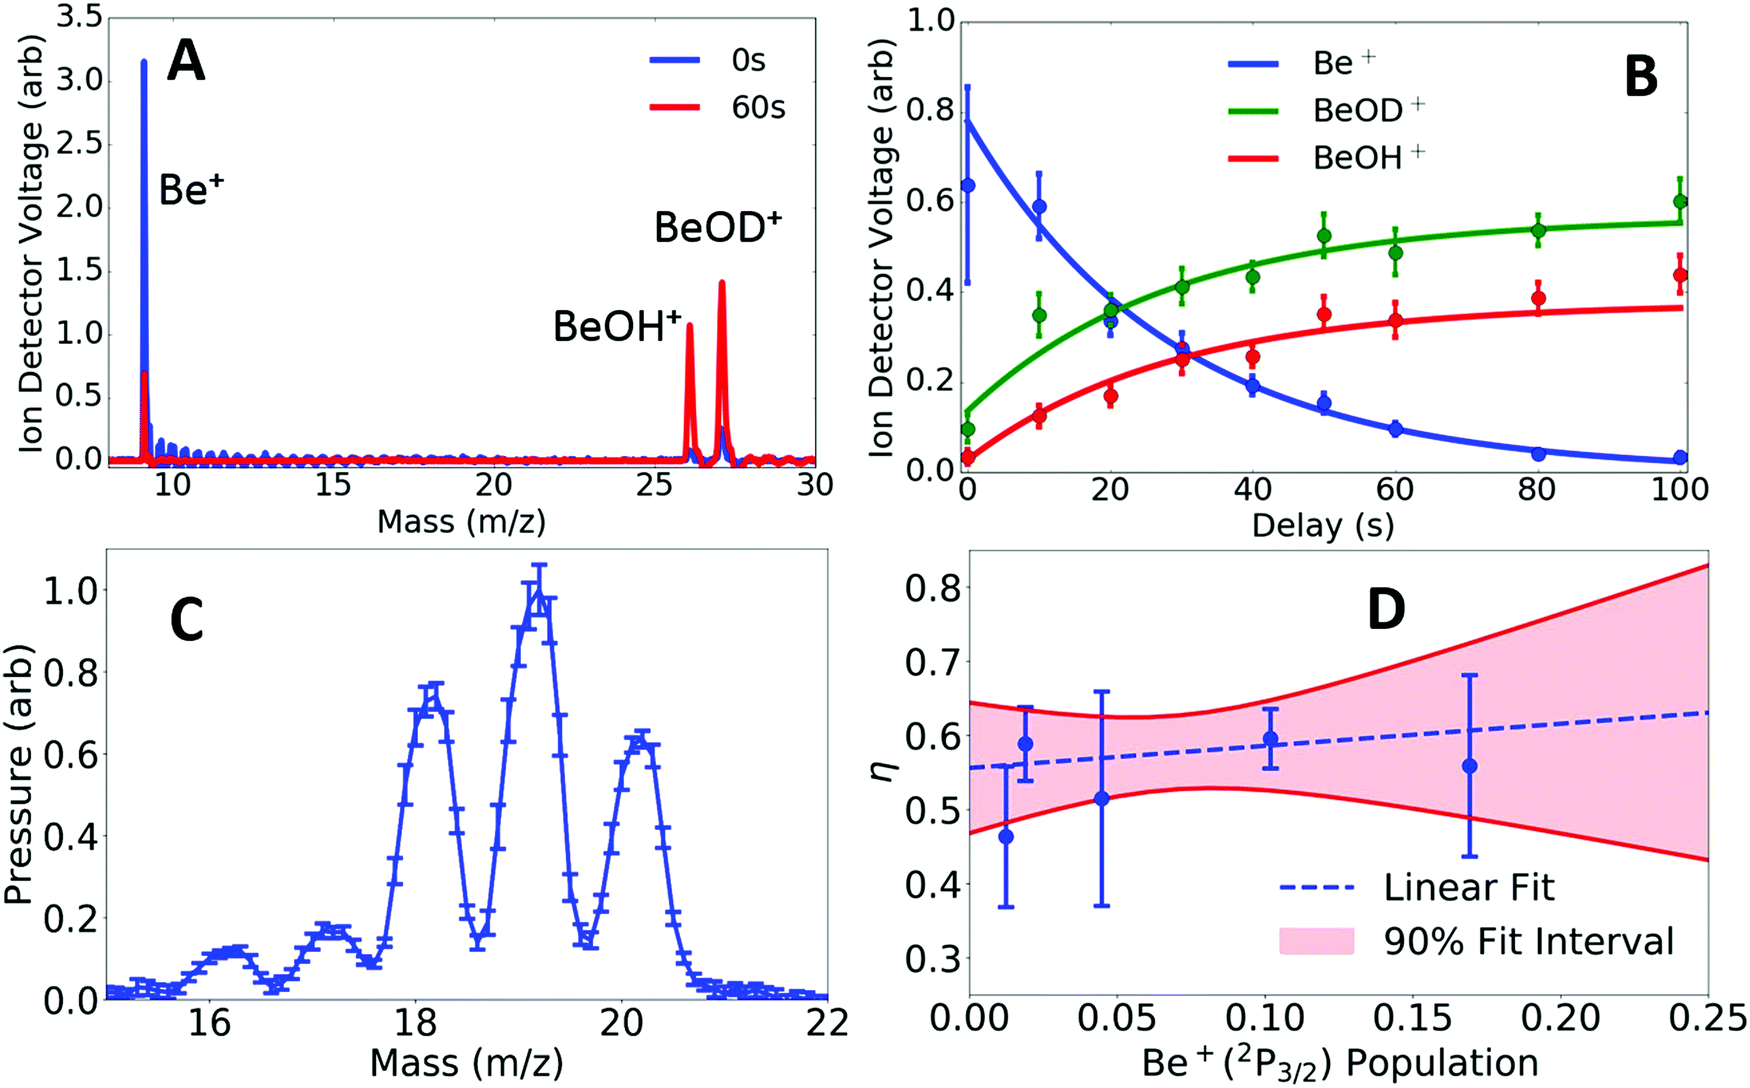
\includegraphics[width=\textwidth]{images/Be_HOD_set.png}
	\caption{(A) A typical TOF signal (5 sample average) at reaction time $t=0$ s and 60 s with $P_{\mathrm{P}} \approx 2\%$. (B) The temporal evolution of \ce{Be+}, \ce{BeOH+}, and \ce{BeOD+} in the trap as a function of reaction time, as well as the solutions of differential equations fitte to the kinetics data with $P_{\mathrm{P}} \approx 2\%$. (C) The RGA signal (8 traces average) gives relative initial \ce{H2O}, \ce{HOD}, \ce{D2O} sample ratio, which is $\rho_1:\rho_2:\rho_3=(1.00 \pm 0.02):(2.45 \pm 0.05):(1.58 \pm 0.02)$. (D) The product fraction for \ce{BeOD+} production ($\eta$) of reactions (\ref{r: Be(S)+HOD->BeOD} and \ref{r: Be(S)+HOD->BeOH}) as a function of \ce{Be+(^2P3/2)} state population. The S-state branching ratio is found to be $\eta_s=0.56 \pm 0.03$, in agreement with the following calculated combined value with different initial H fractions.}
	\label{fig: Be+HOD procedure}
\end{figure}

\begin{figure}
	\centering
	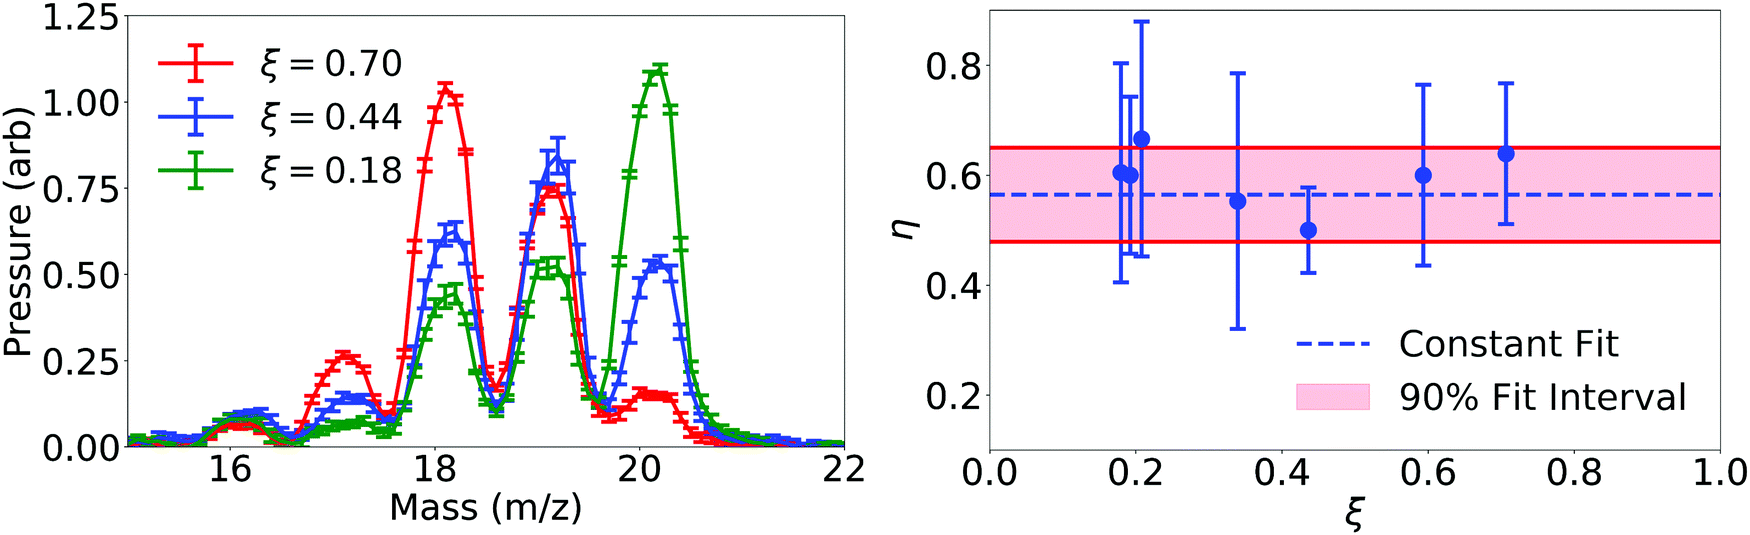
\includegraphics[width=\textwidth]{images/Be_HOD_HOD_frac.png}
	\caption{(left) Averaged (8 traces) RGA analog scan showing peaks at each isotopologue $m/z$. Points around the peak of each isotopologue were averaged for a more accurate partial pressure. (right) The branching ratio $\eta$ of the reaction \ce{Be+ + HOD} into \ce{BeOD+ + H} (with a \ce{Be+} P-state fraction of $P_{\mathrm{P}} \approx 2\%$) as a function of initial H fraction in an HOD, H2O, D2O mixture. Shared fitting the branching ratio $\eta$ with a constant value fit is shown with a weighted average of $\eta = 0.58 \pm 0.14$.}
	\label{}
\end{figure}

\section{Results and Discussion}

Because the \ce{HOD} sample also contains both \ce{H2O} and \ce{D2O}, the product \ce{BeOH+} ($m/z = 26$) has contributions of the reaction of the cation with \ce{H2O}, while \ce{BeOD+} ($m/z = 27$) has contributions from reactions with \ce{D2O}. The reactions of interest are:
\begin{align}
	\ce{Be+(^2S1/2) + H2O & -> BeOH+ + H} \tag{\ref{r: Be(S)+H2O->BeOH}} \\
	\ce{Be+(^2S1/2) + HOD & -> BeOD+ + H} \label{r: Be(S)+HOD->BeOD} \\
	\ce{& -> BeOH+ + D} \label{r: Be(S)+HOD->BeOH} \\
	\ce{Be+(^2S1/2) + D2O & -> BeOD+ + D} \label{r: Be(S)+D2O->BeOD}
\end{align}
Thus, the differential forms and solutions of the reagents and products are solved and shown in \ref{sec: Be+HOD eqs}. The branching ratio $\eta \equiv k_{\ce{BeOD+}}/(k_{\ce{BeOD+}} + k_{\ce{BeOH+}})$ is the fraction of \ce{BeOD+} produced from reaction \ref{r: Be(S)+HOD->BeOD} where $k_j$ is the rate coefficient of species $j$. Solutions to the rate equations \ref{eq: HOD Be(t)}, \ref{eq: HOD BeOD(t)}, and \ref{eq: HOD BeOH(t)} are parameterized by the density measurements of the water isotopologues taken from a RGA, and a least-squares fit is taken over data sets of integrated TOF mass spectra with shared fitting parameters $k_1$, $k_2$, $k_3$, and $\eta$. In order to extract the pure \ce{Be+(^2S1/2)} and \ce{Be+(^2P3/2)}-state branching ratios, the process shown in Figure \ref{fig: Be+HOD procedure}(A)–(C) was repeated at different P-state fractions. The results are shown in Fig. 1(D) along with a least-squares linear-fit (blue line). The vertical intercept of this fit gives $\eta_S = 0.56 \pm 0.03$ for the ground \ce{Be+(^2S1/2)} state reaction, while no conclusive dependence on P-state fractions is found within the confidence intervals. To further verify that our measurement is independent of reagent ratios, we repeated the measurement for different mixtures of \ce{HOD}, \ce{H2O}, and \ce{D2O}, as shown in Fig. 3. The branching ratio of \ce{BeOD+ + H} in reaction \ce{Be+ + HOD} (with 2\% \ce{Be+(^2P3/2)} state population) is consistent over different hydrogen fractions in the gas. The fraction of hydrogen atoms in the chamber ($\xi$) from all water isotopologues is defined by:
\begin{equation}
	\xi = \frac{2 \rho_{\ce{H2O}} + \rho_{\ce{HOD}}}{\rho_{\ce{H2O}} + \rho_{\ce{HOD}} + \rho_{\ce{D2O}}}
\end{equation}
Weighted averaging of the fitted values over different mixtures then gives $\eta = 0.58 \pm 0.14$, $frac{k_2}{k_1} = 0.8 \pm 0.9$, $\frac{k_3}{k_1} = 0.8 \pm 0.9$. Despite the large error bars on the relative rate coefficients, due to the significant covariance of the rate coefficients, $\eta$ is reasonably well determined. To further check our measurement of $\eta$, the process was repeated for shared fits with identical rate coefficients ($k1 = k2 = k3$) yielding $\eta = 0.57 \pm 0.07$. The calculated overall rate coefficients of the \ce{Be+ + D2O} and \ce{Be+ + HOD} reactions are $(2.29 \pm 0.05) \times 10^{-9}$ cm$^3$ molecule$^{-1}$ s$^{-1}$ and $(2.29 \pm 0.05) \times 10^{-9}$ cm$^3$ molecule$^{-1}$ s$^{-1}$, respectively, which are slightly larger than that ($(2.02 \pm 0.04) \times 10^{-9}$ cm$^3$ molecule$^{-1}$ s$^{-1}$)25 of the \ce{Be+ + H2O} reaction. The calculated $k_2/k_1$ and $k_3/k_1$ ratios are $1.13 \pm 0.04$ and $1.13 \pm 0.04$, which are consistent with experimental values of $0.8 \pm 0.9$ and $0.8 \pm 0.9$, respectively. The identical $k_2/k_1$ and $k_3/k_1$ ratios suggests the negligible isotopic effect in the thermal reaction probabilities of the \ce{Be+ + D2O} and \ce{Be+ + HOD} reactions. The branching ratio was determined using the QCT method for the \ce{Be+ + HOD} reaction. Specifically, the calculated branching fraction of \ce{Be+ + HOD} $(\eta)$ is $0.61 \pm 0.02$, which is in good agreement with experimental value $0.58 \pm 0.14$. The branching ratio of the two products (\ce{BeOD+} and \ce{BeOH+}) can be understood in terms of the PST model, which assumes complete energy randomization in the deep intermediate (\ce{BeHOD+}) well. In Fig. 4, the branching fraction for the \ce{BeOD+ + H} channel is plotted as a function of the collision energy, which shows very weak temperature dependence. At the specific collisional temperature 100 K, the fraction obtained by integrating the energy dependent branching ratio with a Boltzmann weight is 0.67, which is in reasonable agreement with the QCT results provided by Hua Guo.\cite{Chen2019}

\subsection{Conclusion}

To summarize, chemical reactions between \ce{Be+(^2S1/2)} and \ce{HOD} have been investigated using an integrated ion trap and highresolution TOF-MS and ZPE corrected QCT calculations on an accurate global PES. Two product channels have been observed and the branching to \ce{BeOD+ + H} is accurately determined to be $0.58 \pm 0.14$. The experimental result is in good agreement with ZPE corrected QCT calculation result ($0.61 \pm 0.02$) as well as close to the statistical PST model (~0.67),\cite{Chen2019} which reveals that the branching to the two product channels is largely due to the availability of different open states in each channel. Since their rate coefficients deviate from the capture limit as reported in our earlier work, it is clear that the \ce{Be+(2S1/2) + H2O/D2O/HOD} reactions have a non-negligible non-statistical component.